\chapter{Resultados Experimentales}


\section{Entorno de pruebas}
Para hacer las pruebas en la placa se ha utilizado la Basys3 de virtex ya que se utiliza la misma en el estudio en el que se basa el proyecto.
El problema que se encontro con el uso de la placa es que la ROM no podria almacenar 650000 filas de valores de punto flotante por lo que se probo un dieciseisavo de las pruebas totales que equivale a 40625.
Porlo que, para hacer la prueba con todos los samples, se requiere utilizar una FPGA con mas recursos como la Virtex-7 VC709 Evaluation Platform.

\begin{figure}[h]
	\centering
	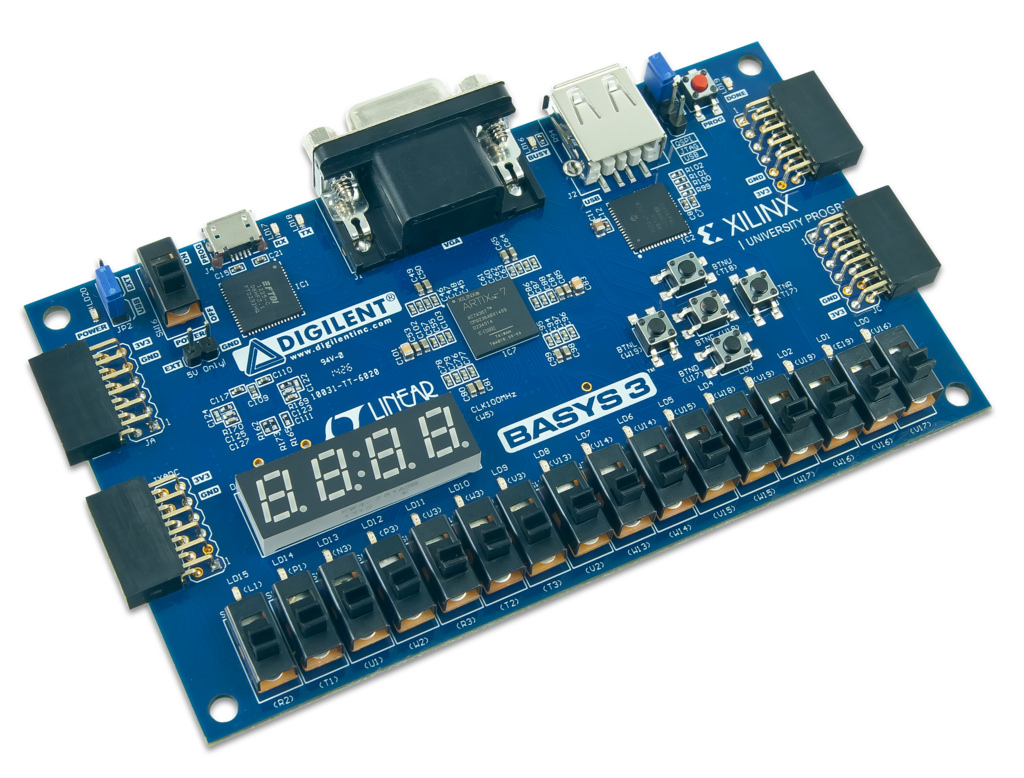
\includegraphics[width=0.6\textwidth]{./Images/img_introduccion/Basys3.jpg}
	\caption{Basys3 Artix-7 FPGA}
	\label{fig:Basys3}
\end{figure}

\section{Consumo}
	Para evaluar el consumo se tendra en cuenta los resultados sacados del análisis de síntesis, del reporte de timing y de el reporte de power de el modulo principal que contiene el modulo de filtrado de señal,
	el módulo de deteccion de picos y el modulo de deteccion de arritmias. 
	
	\begin{figure}[h!]
		\centering
		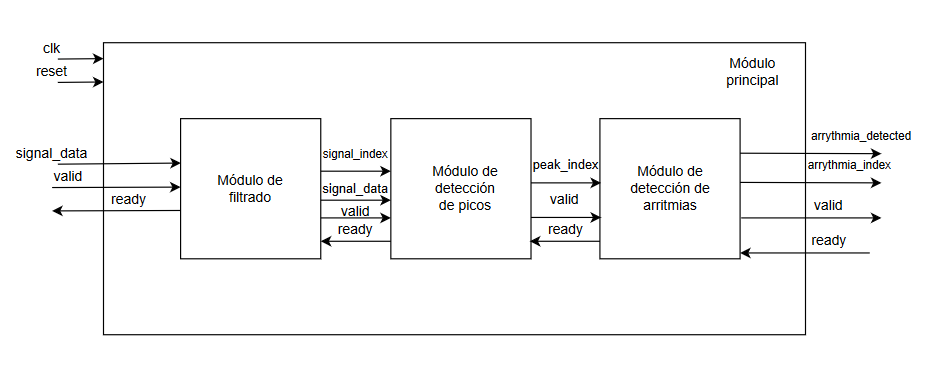
\includegraphics[width=0.99\textwidth]{./Images/img_res_experimentales/diagramaGeneral.png}
		\caption{Diagrama principal de todos los modulos a evaluar}
		\label{fig:Diagramaasmfiltrado}
	\end{figure} 

\subsection{Análisis de síntesis}

	En el análisis de síntesis podemos ver las sigueintes caracteristicas:

	\begin{itemize}
		\item Luts as logic: 195
		\item Luts as memory: 0
		\item Slice registers: Hay 279 slice registers de los cuales todos son flip flops y no hay ningun latch por la arquitectura 
		seguida en la creacion del programa haciendo que al pasar de estado se cambien todas las señales nuevas por las actuales
		\item No se ha usado ningún DSP
		\item No se ha usado ninguna block RAM tile
		\item Hay un total de 474 total slices
		\item La frecuencia de funcionamiento configurada en el .xdc es de 640800 pero para las pruebas se usara una frecuencia de 540000
	\end{itemize}

	La frecuencia de funcionamiento se ha calculado segun la referencia de el articulo \cite{desai2021low} que nos indica que las muestras van a 360sps (samples per second) 
	por lo que es equivalente a 360Hz. Tambien se calcula el numero de ciclos que tarda en ejecutarse el modulo de filtrado que resulta ser el mas critico 
	de todos, este da un total de 1780 ciclos pero para hacer las pruebas se usaran 1500 ciclos. Si se multiplican ambos valores da una frecuencia de 540000 
	cuyo periodo es de 1851,85 que redondeando es de 1852. En el xdc se pone lo siguiente:

\lstset{language=VHDL, breaklines=true, basicstyle=\footnotesize}
\begin{lstlisting}[frame=single]
## Clock signal
set_property PACKAGE_PIN W5 [get_ports clk]							
	set_property IOSTANDARD LVCMOS33 [get_ports clk]
	create_clock -add -name sys_clk_pin -period 1852.00 -waveform {0 926} [get_ports clk]
\end{lstlisting}

El waveform oscila desde 0 a 926 para que sea simétrico.

\subsection{Análisis de timing}
	En el análisis de timing se vera cual es el worst negative slack y se calculara la frecuencia minima necesaria. Este reporte de timing muestra lo siguiente.

	\begin{figure}[h!]
		\centering
		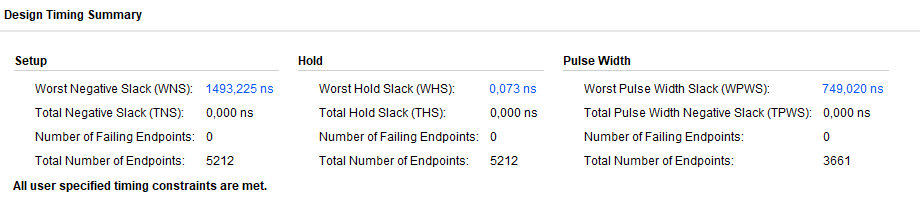
\includegraphics[width=0.9\textwidth]{./Images/img_res_experimentales/reportetiming.png}
		\caption{Imagen que muestra el reporte de timing generado}
		\label{fig:reporteTiming}
	\end{figure} 

	Para calcular la frecuencia minima necesaria se resta la frecuencia actual menos el worst negative slack dando como resultado 6,49 ns de frecuencia mínima de funcionamiento. 

\subsection{Análisis de power}

	En el análisis de power se evalua la potencia que necesita la FPGA para poder llevar a cabo las instrucciones.

	\begin{figure}[h!]
		\centering
		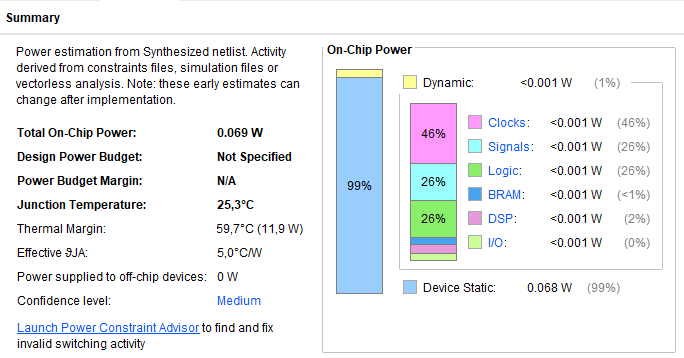
\includegraphics[width=0.6\textwidth]{./Images/img_res_experimentales/reportepower.png}
		\caption{Imagen que muestra el reporte de power generado}
		\label{fig:reportePower}
	\end{figure} 

	Comparando este proyecto con otros estudios, por ejemplo con el de caracterizacion de señales usando polinomios de hermite presentan unos resultados de dynamic power de 28mW.
	Sin embargo, el dynamic power de este proyecto es menor que 0,001W.








	